\clearpage

\section{결과 관리와 활용}\label{sec:ops}

\subsection{캠페인 진행}

여러 시험의 묶음을 캠페인이라 한다. 그림~\ref{fig:campaign}은 하나의 캠페인이 진행되는 흐름이다.

\begin{figure}[H]
\centering
\begin{tikzpicture}[every node/.style={font=\footnotesize}]
  \node[box, minimum width=26mm] (b) at (0,0)      {시험 입력 생성\\\scriptsize 시드 기반};
  \node[box, minimum width=26mm] (c) at (3.6,0)    {대상 연결\\\scriptsize 또는 대기 중인 충전기};
  \node[hot, minimum width=28mm] (d) at (7.4,0)    {시험 실행\\\scriptsize 메시지 송수신};
  \node[box, minimum width=28mm] (o) at (11.2,0)   {판정\\\scriptsize 등급 · 근거};
  \node[box, minimum width=28mm] (e) at (11.2,-1.8){결과 기록\\\scriptsize 판정 · 근거 · 재현 정보};
  \node[ext, minimum width=28mm] (g) at (7.4,-1.8) {중단 조건 확인\\\scriptsize 사용자 중지 · 응답 불능};
  \node[ext, minimum width=26mm] (h) at (3.6,-1.8) {캠페인 종료};
  \draw[arr] (b) -- (c);
  \draw[arr] (c) -- (d);
  \draw[arr] (d) -- (o);
  \draw[arr] (o) -- (e);
  \draw[arr] (e) -- (g);
  \draw[arr] (g) -- node[lbl, right]{다음 시험} (d);
  \draw[arr] (g) -- node[lbl, above]{완료} (h);
  \draw[arr, dashed] (c) -- node[lbl, left, align=right]{연결 실패 시\\원인을 결과로 남김} (h);
\end{tikzpicture}
\caption{캠페인 진행 흐름}
\label{fig:campaign}
\end{figure}

시험을 만들 수 없거나, 대상에 연결할 수 없거나, 시험할 충전기가 선택되지 않은 경우에도 캠페인은 조용히 끝나지 않고 그 원인을 설정 오류 또는 잘못된 테스트 결과로 남긴다.
사용자는 결과 화면에서 ``왜 아무 결과도 없는지''를 바로 확인할 수 있다.

\subsection{결과 기록과 재현}

각 시험 결과에는 판정 등급, 이유, 신뢰도, 근거와 함께 주고받은 메시지 원문, 세션 상태의 흐름, 그리고 시험 입력 자체(단계, 변형, 시드)가 기록된다.
입력 생성이 시드에 대해 결정적이므로, 같은 설정과 시드로 캠페인을 다시 실행하면 같은 입력이 재현된다.
잠재 이슈가 발견되면 기록된 메시지 순서와 시드를 개발자에게 전달하여 로컬 환경에서 동일한 상황을 재현할 수 있다.

웹 화면의 결과 목록(그림~\ref{fig:ui-results})은 판정 등급별 건수를 위쪽에 요약하고, 그 아래에 시험별 결과를 나열한다.
결과, 테스트 유형, 메시지, 신뢰도로 목록을 걸러 볼 수 있으며, 결과 전체를 파일로 내려받을 수 있다.
각 결과의 \textbf{증거 열기}를 누르면 그림~\ref{fig:ui-detail}의 상세 화면으로 이동한다.

\begin{figure}[H]
    \centering
    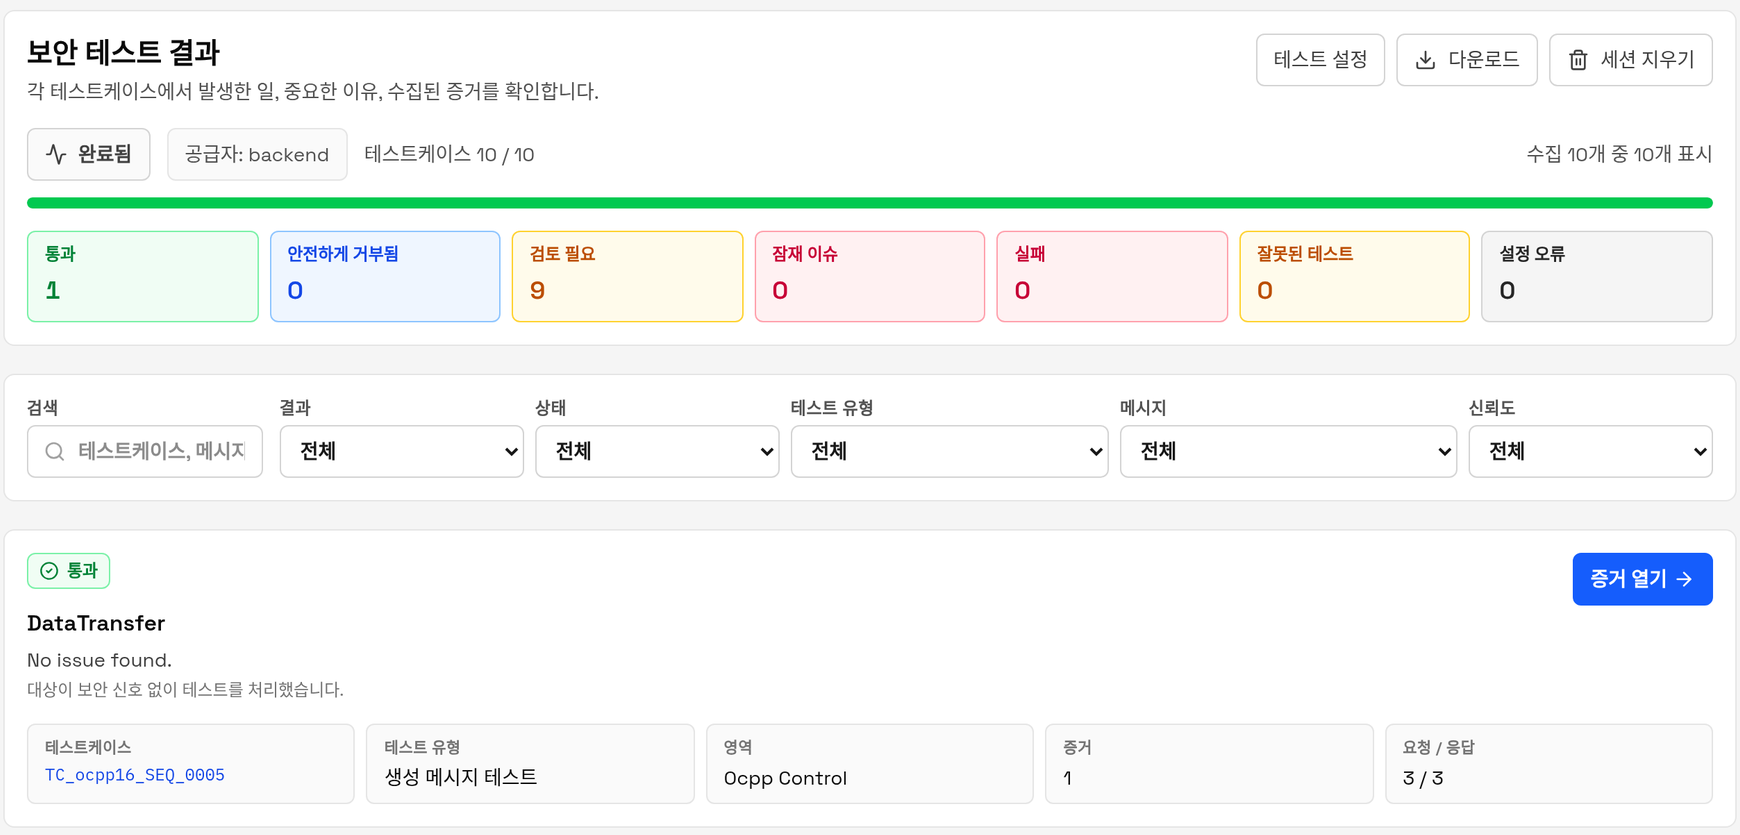
\includegraphics[width=\textwidth]{screenshots/ui03_results_c.png}
    \caption{웹 화면: 결과 목록과 판정 요약}
    \label{fig:ui-results}
\end{figure}

그림~\ref{fig:verdict-dist}는 개발 기간 동안 OCPP 1.6 대상으로 누적된 시험 결과 829건의 판정 분포이다.
여러 차례의 시험 실행이 합쳐진 값이므로 특정 대상의 보안 수준을 나타내지는 않는다.
다만 정책 프로파일 없이 시험하면 결론을 보류한 검토 필요 판정이 많아진다는 점, 그리고 판정 기준이 잠재 이슈를 보수적으로 산출한다는 점(5건, 모두 잘못된 커넥터 번호로 트랜잭션이 생성된 경우)을 보여 준다.

\begin{figure}[H]
\centering
\begin{tikzpicture}
\begin{axis}[
    xbar, bar width=9pt,
    width=0.8\textwidth, height=6.2cm,
    xmin=0, xmax=600,
    axis x line*=bottom, axis y line*=left,
    xmajorgrids, grid style={ksgray!25},
    major x tick style={draw=none},
    symbolic y coords={잠재 이슈,설정 오류,실패,통과,안전하게 거부됨,검토 필요},
    ytick=data,
    yticklabel style={font=\footnotesize},
    xticklabel style={font=\footnotesize, ksgray},
    xlabel={결과 건수}, xlabel style={font=\footnotesize, ksgray},
    nodes near coords, nodes near coords style={font=\footnotesize, black},
    enlarge y limits=0.12,
]
\addplot[draw=none, fill=ksblue] coordinates {
    (523,검토 필요) (241,안전하게 거부됨) (26,통과) (18,실패) (16,설정 오류) (5,잠재 이슈)
};
\end{axis}
\end{tikzpicture}
\caption{OCPP 1.6 누적 시험 결과의 판정 분포 (829건)}
\label{fig:verdict-dist}
\end{figure}

\subsection{한계 및 향후 과제}

\begin{itemize}
    \item \textbf{ISO 15118 인코딩}: 현재 기본 인코더는 시험용 간이 구현이므로, 실제 충전기 측 제어기를 시험하려면 실제 EXI 구현의 연결이 필요하다.
    \item \textbf{암호화 통신}: 충전기 시험의 TLS 기반 보안 프로파일은 구조만 마련되어 있으며, 인증서 관리 기능이 추가되어야 한다.
    \item \textbf{응답 내용 검증 범위}: 응답 내용의 세부 검증은 핵심 메시지에 한정되어 있으며, 나머지는 형식과 상태 불변식으로 판정한다.
    \item \textbf{직접 재전송}: 기록된 시험을 그대로 다시 보내는 기능은 아직 없으며, 현재는 같은 설정과 시드로 캠페인을 다시 실행하여 재현한다.
    \item \textbf{커버리지 기반 퍼징}: 블랙박스 환경을 전제로 하므로 대상 내부의 실행 경로 정보를 활용하지 않는다.
\end{itemize}
